\subsubsection{Clustering}
\label{subsec:03clustering}
Der letzte Schritt der Bildverarbeitung besteht aus dem Clustering. Das Ziel ist die Bestimmung der Tiefe der Person aus der getrackten Bounding-Box mit m�glichst simplen und somit rechensparsamen Ans�tzen. Um �berhaupt Tiefeninformationen zu erhalten, wird ab diesem Schritt das Tiefenbild der Kinect-Kamera verwendet. Im ersten Schritt wird die Bounding-Box nach bestimmten Kriterien �berpr�ft, um den Voraussetzungen des an das Farbbild angepasste Tiefenbild zu gen�gen. Die Voraussetzungen ergeben sich aus dem schwarzen Bereichen an den R�ndern des Tiefenbildes, die durch dessen Verzerrung entstehen. Weiterhin werden invalide Tiefenbestimmungen aus dem Tiefenbild gefiltert, um aussschlie�lich brauchbare Werte in den n�chsten Verarbeitungsschritten zu ber�cksichtigen. \\
Aus den Tiefenpixel, die sich innerhalb der Bounding-Box befinden, wird nun der Mittelwert gebildet und anschlie�end eine Maske erstellt, die ausschlie�lich Pixel unterhalb des Mittelwertes ber�cksichtigen:
\begin{align}
Mask(x,y)=\left\{\begin{matrix}
1 \ \ \ \ if \ BBox(x,y) < \frac{1}{N_{x}+N_{y}} \sum_{x=0}^{N_{x}}\sum_{y=0}^{N_{y}}BBox(x,y)  \\ 
0 \ \ \ \ if \ BBox(x,y) > \frac{1}{N_{x}+N_{y}} \sum_{x=0}^{N_{x}}\sum_{y=0}^{N_{y}}BBox(x,y)
\end{matrix}\right.
\end{align}
$Mask(x,y)$ und $BBox(x,y)$ beschreiben die Pixel der Maske bzw. Bounding-Box an der Stelle $(x,y)$ und $N_{x}$ bzw. $N_{y}$ die Anzahl der Pixel in der jeweiligen Richtung. Der Gedanke hinter diesem Vorgehen ist, dass die Bounding-Box im Normalfall nur die Person und den Hintergrund enth�lt. Sollte dennoch zus�tzlich ein Hinderniss in der Bounding-Box auftauchen, w�rde es nur einen kleinen Teil im Auschnitt ausmachen und somit die Maske kaum verf�lschen. In Abbildung \ref{fig:Maskierung} wird die Maskierung anhand eines Beispielbildes gezeigt.\\
Anschlie�end werden die Tiefenpixel aus dem Tiefenbild, die sich innerhalb der Maske befinden, erneut gemittelt, um die gemittelte Tiefe der verfolgten Person zu erhalten. Zusammen mit dem Mittelpunkt des Detektionsfensters ergeben sich daraus die 3D-Koordinaten $\vec{p} = [p_x, p_y, p_z]^T$ der Person.
\begin{figure}[h]
	\centering
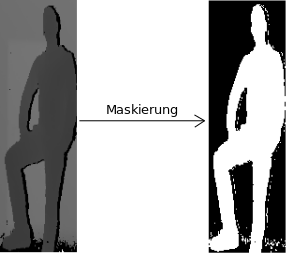
\includegraphics[width=0.4\textwidth]{pics/Maskierung.png}
	\caption{Die Maskierung der Bounding-Box des Tiefenbildes}
	\label{fig:Maskierung}
\end{figure} \\
